\section{Introduction}
Deep learning models have proved remarkably successful for information retrieval (IR) in recent years. The goal herein is to 
rank among a collection of documents the top relevant ones given a query. By utilising deep neural networks, these models aim to learn a function that can automatically extract matching patterns from two pieces of text, that is the query and the document, end-to-end in place of hand-crafted features. 

In general, there are two categories of neural matching architectures. One is called representation-based matching, which projects the query and document into the same low-dimensional semantic space and scores according to their similarity. Examples include DSSM \cite{huang2013learning}, ARC-I \cite{hu2014convolutional}, and CDSSM \cite{shen2014latent}. Another is called interaction-based matching, which learns relevant patterns directly from the interaction signals between the query and the document. Examples include DRMM \cite{guo2016deep}, KNRM \cite{xiong2017end}, 
and PACRR \cite{hui2017pacrr,hui2018co}. While the first category primarily concentrates on the semantics, the second emphasises more on the relevance. As discussed in \cite{guo2016deep}, there are significant differences between semantic matching and relevance matching. The latter is naturally more suitable for ad-hoc retrieval since the term-level query-document interaction provides more specific matching signals than the ensemble of semantic representations. 

\begin{figure}[t]
	\centering
	\subfigure[Query-document pair from Robust04]
	{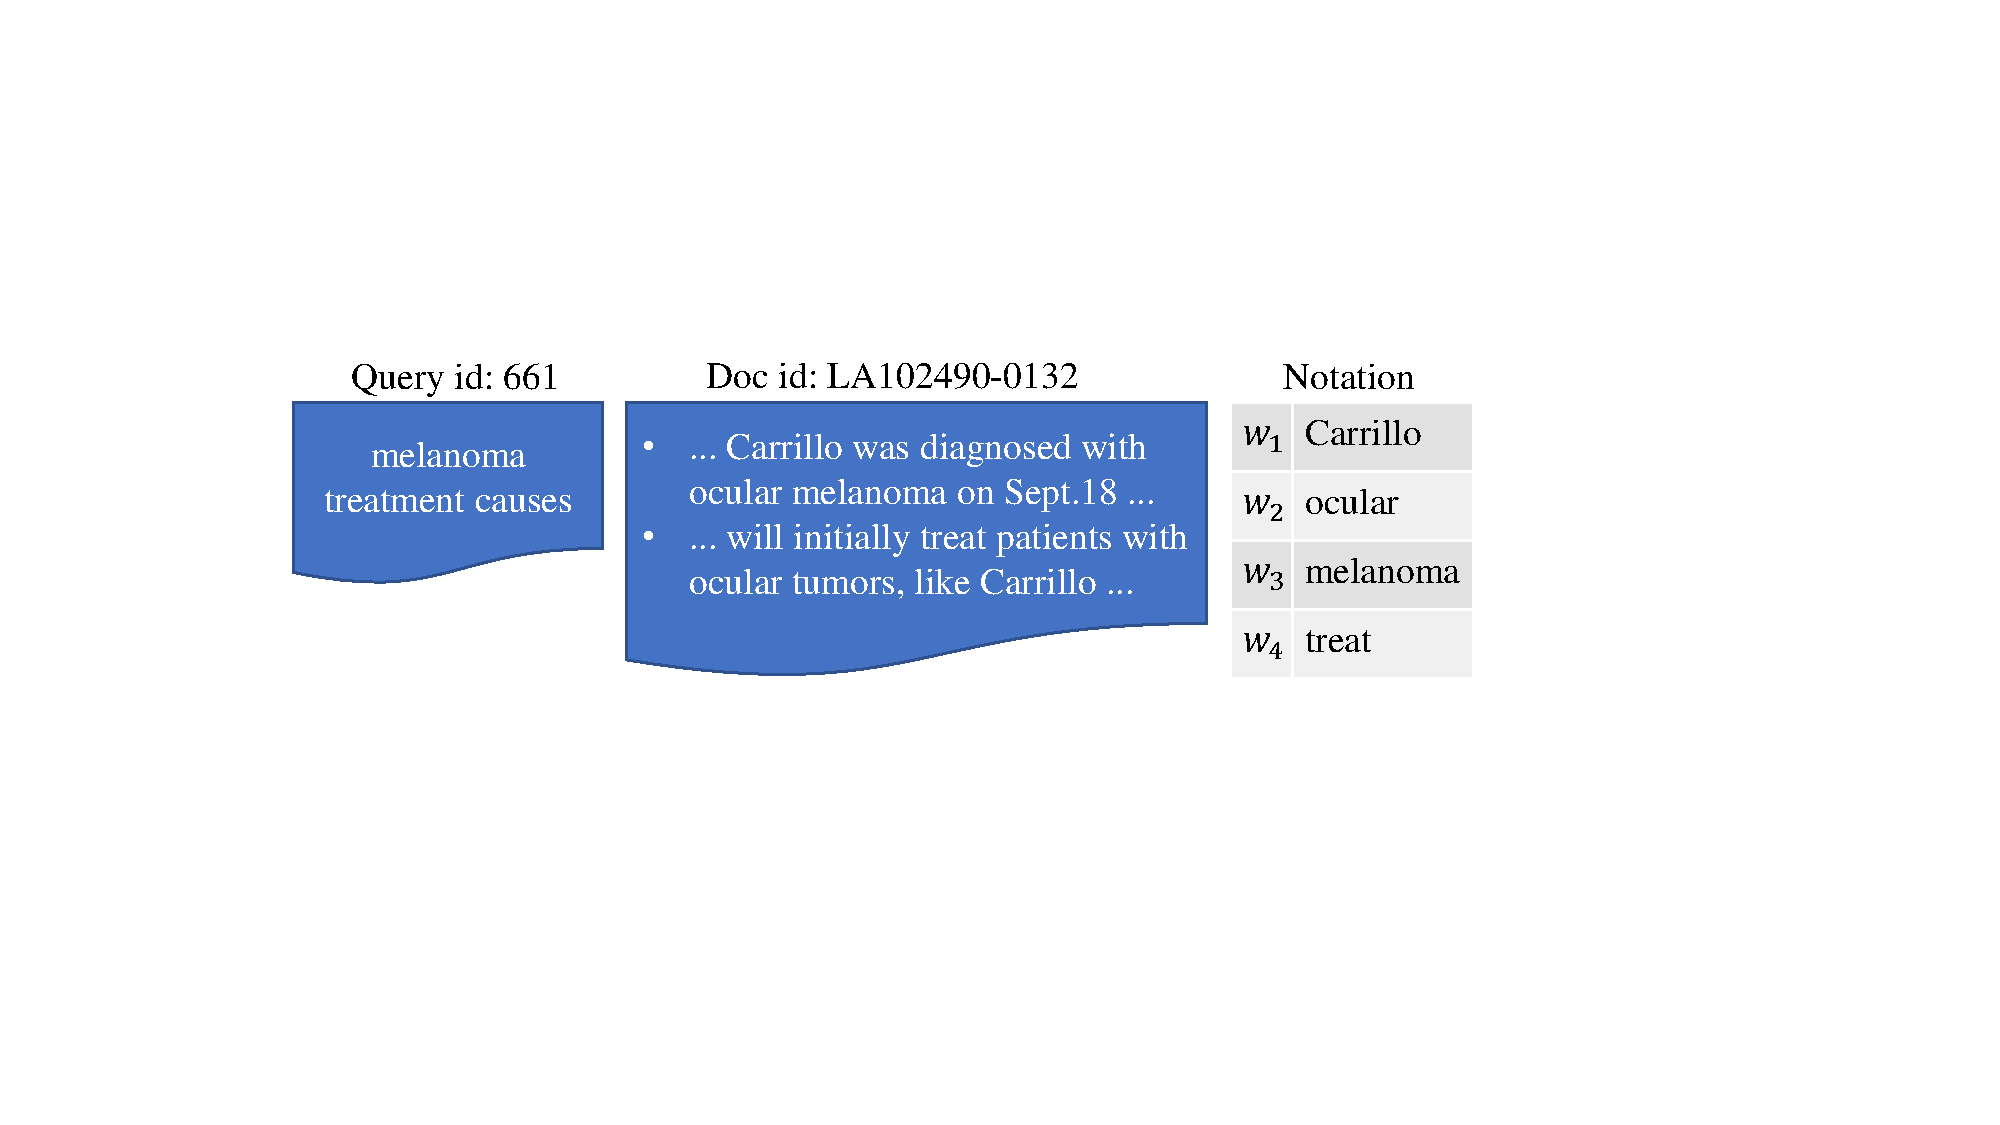
\includegraphics[scale=0.4]{./pics/example.pdf}
	\label{fig:1a}}
	\subfigure[A local context scheme]
	{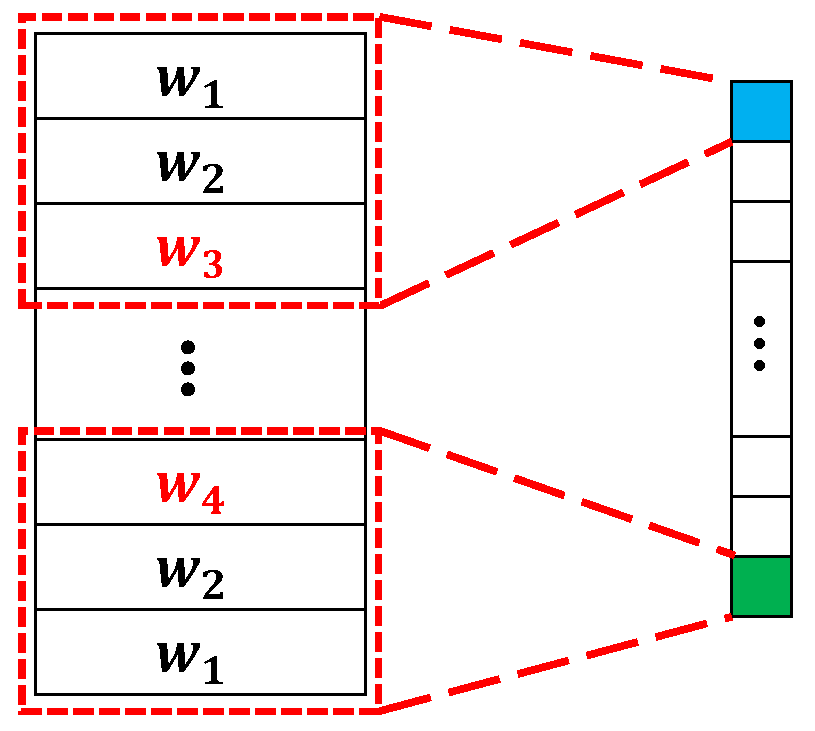
\includegraphics[scale=0.24]{./pics/cnn.pdf}
	\label{fig:1b}}
	\subfigure[A graph-based context scheme]
	{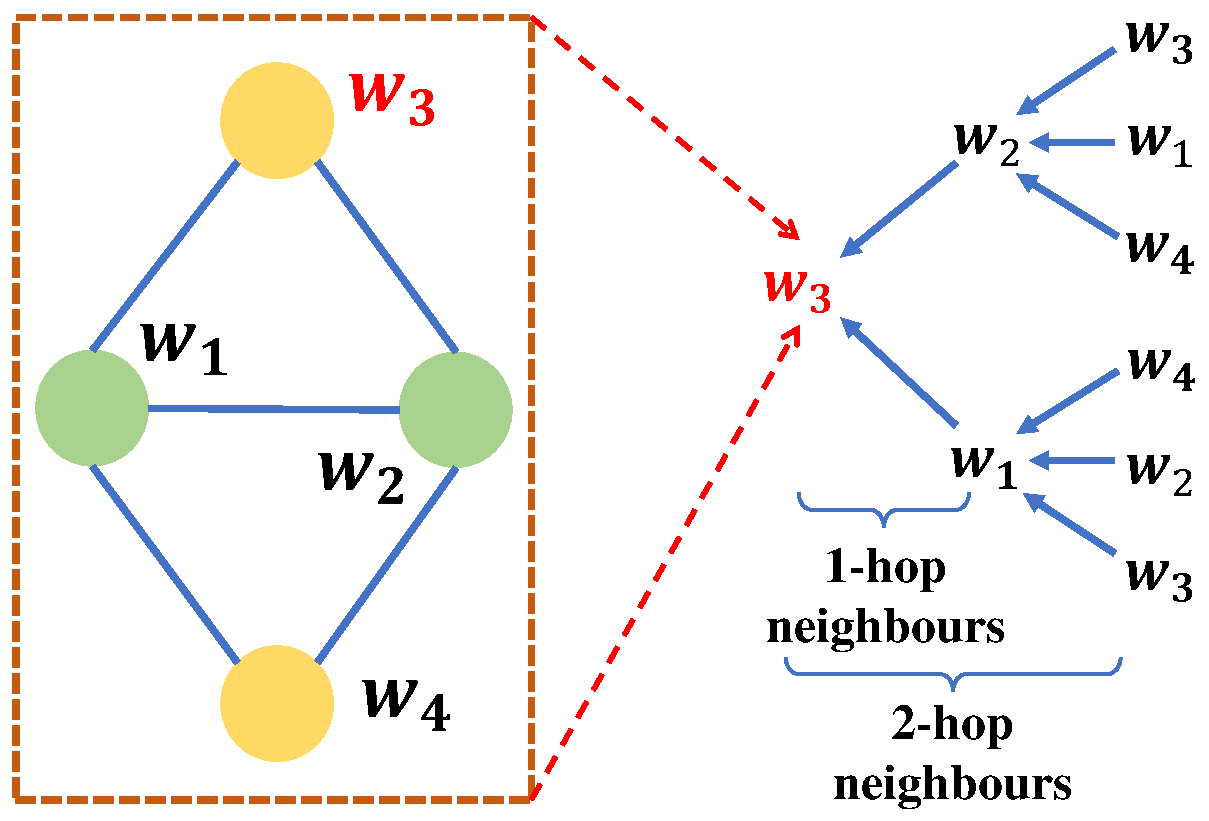
\includegraphics[scale=0.22]{./pics/gnn.pdf}
	\label{fig:1c}}
	\label{fig:1} 
	\caption{An example of relevant query-document pair with two sentences far apart in the document (some words omitted). Local context scheme fails to discover the long-distance matching patterns due to the restriction of context. Graph-based context scheme works since words ``Carrillo'' and ``ocular'' play an important bridge role to connect ``melanoma" and ``treat" together.}
\end{figure}

In addition to the term-level query-document interaction, the document-level word relationships are also essential for relevance matching yet less explored so far. Taking Figure \ref{fig:1a} as an example, when searching with the query ``melanoma treatment", the retrieved document is expected to be highly relevant to them as a whole rather than to any single of ``melanoma" or ``treatment". However, query phrases do not always appear exactly in the document. It occurs more frequently that they (or their synonyms) distribute non-consecutively in any passage and still reserve a long-distance contextual association. Many works that rely on local word sequences \cite{pang2016text,pang2017deeprank,hui2017pacrr} fail to discover such dependencies due to the restriction of context, as illustrated in Figure \ref{fig:1b}. They, therefore, lead to a low score. We argue that these traditional term-level interactions are insufficient for relevance matching, and document-level relationships should be considered 
explicitly and concurrently. 

With recent researches towards graphs for natural language processing (NLP), \citet{yao2019graph} and \citet{zhang2020every} have demonstrated the usage of graph neural networks as a language model and their benefit in capturing long-distance word dependencies. Such graph structures could help search for non-consecutive phrases while maintaining their contextual meaning. For instance, Figure \ref{fig:1c} illustrates a connected graph for the document, where the words ``ocular" and ``Carrillo" nearby ``melanoma" and ``treat" could serve as a bridge connecting them. The query phrase emerges integrally in this way, resulting in a strong matching signal. Given the above, we aim to leverage the graph neural networks to expand the respective field through a flexible text format and assist in the document-level word relationships for ad-hoc retrieval.

In this work, we propose a \textbf{G}raph-based \textbf{R}elevance \textbf{M}atching \textbf{M}odel (GRMM) to resolve the match problem of long-distance terms. For a pair of query and document, we first transform the document into the graph-of-word form \cite{rousseau2015text}, where nodes are unique words, and edges are their co-occurrent linkages. Each node feature is assigned with the interaction between its word and query terms. Instead of raw word features, the interaction vector contains substantial matching signals, which is critical for relevance matching. We then apply graph neural networks to propagate these matching signals on the document graph. Thus the query-document interaction and intra-document word relationships can be modeled jointly. Finally, to estimate a relevance score, we adopt a $k$-max-pooling strategy for each query term to filter out irrelevant noisy information and feed their features into a dense neural layer.

We validate GRMM on two representative ad-hoc retrieval benchmarks, where empirical results show the effectiveness and rationality of GRMM. We also compare our model with BERT-based method, where we find that BERT potentially suffers from the same problem when the document becomes long. 

To sum up, the contributions of this work are as follows:
\begin{itemize}
	\item We point out the importance of explicitly considering long-distance word relationships for ad-hoc retrieval to enhance the query search.
	\item We propose a novel graph-based relevance matching model to address word relationships over the document, which can learn term-level and document-level matching signals jointly.
	\item We conduct comprehensive experiments to examine the effectiveness of GRMM and understand its working principle.
\end{itemize}